\documentclass[../main.tex]{subfiles}
\graphicspath{{\subfix{../images/}}}
\begin{document}

\begin{definition}
    Nechť $X$ je metrický prostor, 
    $\{S(t)\}_{t\in\square}$ je dynamický systém na $X$.
    Pak: 
    \begin{enumerate}
        \item $X$ se nazývá fázový prostor 
        \item Pro $x_0 \in X $ množina $\{S(t)x_0\}_{t\in\square}$ se nazývá \textbf{trajektorie} procházející bodem $x_0 \in X$
        \item Bod $x^\star \in X$, pro který $S(t)x^\star = x^\star, \forall t\in \square$, se nazývá \textbf{pevný bod} dynamického systému
        \item Množina $A\subset X$, pro kterou $S(t)A=A, \forall t \in \square$, se nazývá \textbf{invariantní}
        \item Pevný bod $x^\star\in X$ je \textbf{stabilní}, pokud $\left(\forall H^{(1)}_{x^\star} \text{okolí}\right)\left(\exists H^{(2)}_{x^\star} \text{okolí}\right)$\break
        $\left(\forall x_0\in H^{(2)}_{x^\star}\right)\left(\forall t \in \square, t>0\right)\left(S(t)x_0\in H^{(1)}_{x^\star}\right)$
        \item Pevný bod $x^\star \in X$ je \textbf{nestabilní}, pokud není stabilní
        \item Pevný bod $x^\star \in X$ je asymptoticky stabilní, pokud je stabilní a navíc $\left(H^{(3)}_{x^\star} \text{okolí}\right)\left(\forall x_0 \in H^{(3)}_{x^\star}\right)\left(S(t)x_0 \overset{\square \rightarrow t, t \rightarrow \infty}{\longrightarrow} x^\star\right)$
    \end{enumerate}
\end{definition}

\begin{definition}
    Pro zkrácení zápisu místo okolí budeme psát $\in \mathcal{J}_X$, přesný vzhled záleží na topoplogii.
\end{definition}


\begin{example}
    Zadání je:
    \begin{equation}
        \dot{x} = ax, a\in \mathbb{R}, x(0)= x_0
    \end{equation}

    Řešení má tvar $x(t) = e^{ta}x_0, t\in \mathbb{R}$, pak $X=\mathbb{R}, S(t) = e^{ta}$. Ověříme 
    \begin{enumerate}
        \item $S(t): \mathbb{R} \rightarrow \mathbb{R}$ jako násobení je spojité 
        \item $S(0)=1 \implies S(0) = \identity$
        \item $S(s+t) = e^{(s+t)a} = e^{sa}e^{ta}= S(s)S(t) = S(s)\circ S(t)$
    \end{enumerate}

    Z toho dostáváme že zadání generuje dynamický systém na $\mathbb{R}$
\end{example}

\begin{example}
    Zadání je 
    \begin{equation}
        \dot{x} = \mathbb{A}x, \mathbb{A}\in \mathbb{R}^{n,n}, x(0)= x_0
    \end{equation}
    
    Řešení je $x: \mathbb{R} \rightarrow \mathbb{R}^n$ a má tvar
    $x(t) = e^{t \mathbb{A}}x_0, t\in \mathbb{R}$, kde $e^{t\mathbb{A}} = \sum_{k=0}^{\infty} \frac{1}{k!} \left(t \mathbb{A}\right)^k$.

    Z toho máme, že $S(t) = e^{t\mathbb{A}}$. Ověříme že se jedná o dynamický systém
    \begin{enumerate}
        \item $S(T)$ je spojité, neboť $S(t)$ funguje jako násobení matice a vektoru což je spojitá operace
        \item $S(0) = \mathbb{I}$, což je identita na $\mathbb{R}^n$
        \item $S(s+t) = S(s) \circ S(t)$, dle vlastnoti $e^{(s+t)\mathbb{A}} = e^{s\mathbb{A}}e^{t\mathbb{A}}$
    \end{enumerate}

\end{example}

\begin{example}
    Zadání je 
    \begin{equation}
        \dot{x} = 1+x^2, x(0)=x_0
    \end{equation}
    To je separovatelná rovnice s řešením 
    \begin{equation}
        \int_{0}^{t} \frac{\dot{x}(t)dt}{1+(x(t))^2} = \int_0^t 1 dt
    \end{equation}
    \begin{equation}
        \int_{x_0}^{x(t)} \frac{dy}{1 + y^2} = t 
    \end{equation}
    \begin{equation}
        \arctan(x(t)) - \arctan(x_0) = t
    \end{equation}

    tedy 
    \begin{equation}
        x(t) = \tan(t + \arctan(x_0)), x_0 \in \mathbb{R} \implies \arctan(x_0)\in (-\pi/2, \pi/2)
    \end{equation}

    Z toho máme maximální  rozsah $t\in \left(- \frac{\pi}{2} - \arctan(x_0), \frac{\pi}{2} - \arctan(x_0)\right)$.

    Zadání tedy negeneruje dynamický systém.

\end{example}


\begin{example}
    \textbf{Hénonů atraktor}

    \begin{equation}
        x^1_{n+1} = x^2_n + 1 - a\left(x^1_n\right)^2, x^2_{n+1} = bx^1_n
    \end{equation}
    Navíc $a=1.4, b=0.3$

    Generujeme posloupnost $\left\{\binom{x_n^1}{x_n^2}\right\}_{n=1}^\infty$ v $\mathbb{R}^2$,
    tj $X = \mathbb{R}^2$

    Diskretní dynamický systém
    \begin{enumerate}
        \item $F\binom{x^1}{x^2} = \binom{  x^2 + 1 - a(x^1)^2 }{bx^1}$ je spojité.
        \item $F^[0] = \identity$
        \item $F^{[m+n]} = F^{[m]}\circ F^{[n]}$
    \end{enumerate}

\end{example}


\begin{example}
    Použijeme příklad 2 (ten s maticí ) pro $n=2$, tj. $X=\mathbb{R}^2$
    
\begin{enumerate}
    \item Nejdříve vezměme matici 
    \begin{equation}
        \mathbb{A} = \begin{pmatrix}
            -1 & 0 \\
            0 & 1 
            \end{pmatrix}
    \end{equation}

    Tedy $\dot{X}^1 = - x^1$ a $\dot{x}^2 = x^2$ s řešením $x^1(t) = e^{-t}x^1_0$ a $x^2(t) = e^t x_0^2$

    \begin{center}
        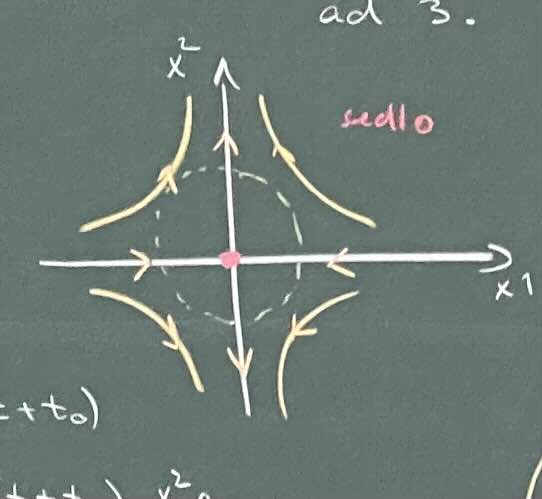
\includegraphics[width=0.5\linewidth]{images/sedlo.jpg}
    \end{center}

    Tedy máme $\mathbb{A}=X$ je invariantní, osy $x^1$ a $x^2$ je invariantní a pevný bod $x^\star = [0,0]$ je nestabilní.


    \item Nyní vezměme matici 
    \begin{equation}
        \mathbb{A} = \begin{pmatrix}
            0 & -1 \\
            1 & 0 
            \end{pmatrix}
    \end{equation}
    Tedy $\dot{X}^1 = - x^2$ a $\dot{x}^2 = x^1$ s řešením $x^1(t) = r_0 \cos(t+t_0)$ a $x^2(t) = r_0 \sin(t+t_0)$
    \begin{center}
        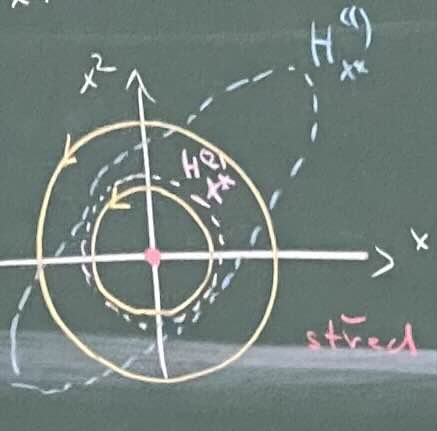
\includegraphics[width=0.5\linewidth]{images/stred.jpg}
    \end{center}

    Máme pevný bod $x^\star = [0,0]$, $A=X$ je invariantní.


    \item Nyní vezměme matici 
    \begin{equation}
        \mathbb{A} = \begin{pmatrix}
            -1 & 0 \\
            0 & -2 
            \end{pmatrix}
    \end{equation}
    Tedy $\dot{X}^1 = - x^1$ a $\dot{x}^2 = -2x^2$ s řešením $x^1(t) = e^{-t}x^1_0$ a $x^2(t) = e^{-2t} x_0^2$

    Po úpravách dostáváme $\frac{x^2(t)}{\left(x^1(t)\right)^2} = \frac{x^2_0}{\left(x_0^1\right)^2}$ a proto 
    $x^2 = \left(x^1\right)^2 \frac{x_0^2}{\left(x_0^1\right)^2}$

    \begin{center}
        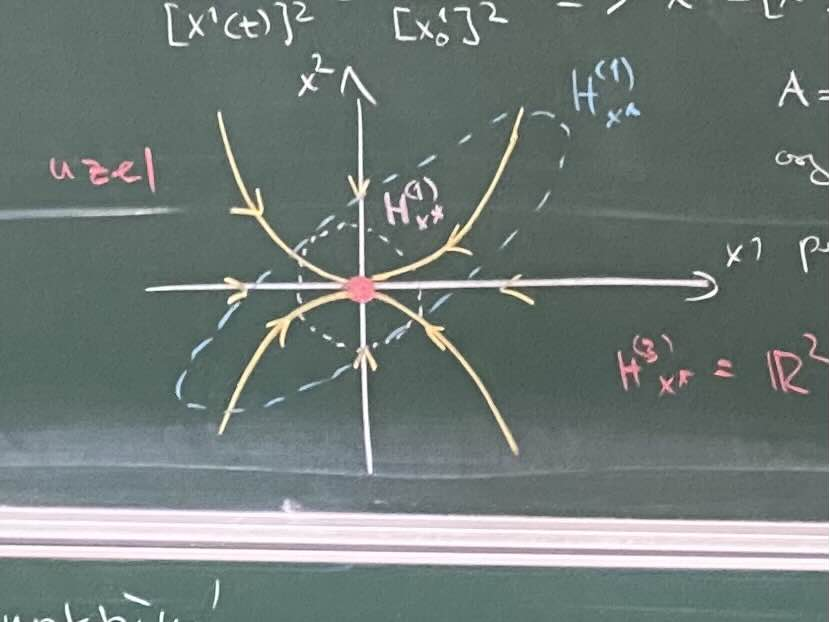
\includegraphics[width=0.5\linewidth]{images/uzel.jpg}
    \end{center}

    $A=X$ je invariantní, osy $x^1, x^2$ jsou invariantní, máme pevný bod $x^\star = [0,0]$

    \item Matice \begin{equation}
        \mathbb{A} = \begin{pmatrix}
            1 & 0 \\
            1 & 1 
            \end{pmatrix}
    \end{equation}
    Tedy $\dot{X}^1 = - x^1$ a $\dot{x}^2 = x^1 + x^2$ s řešením $x^1(t) = e^{t}x^1_0$ a $x^2(t) = (x_0^1 t + x_0^2)e^t $
    \begin{center}
        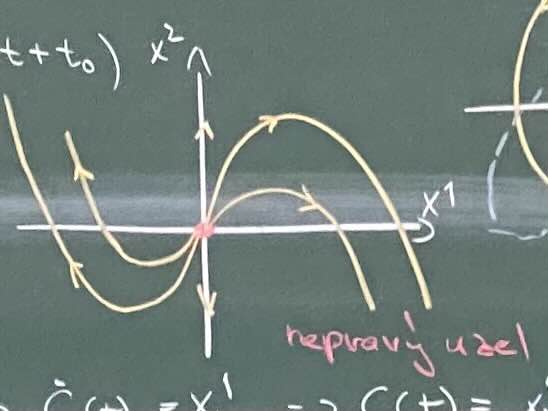
\includegraphics[width=0.5\linewidth]{images/nepravy-uzel.jpg}
    \end{center}

    Pevný bod $x^\star=[0,0]$ je nestabilní


    
    \item Matice \begin{equation}
        \mathbb{A} = \begin{pmatrix}
            1 & -1 \\
            1 & 1 
            \end{pmatrix}
    \end{equation}
    Tedy $\dot{X}^1 = x^1 - x^2$ a $\dot{x}^2 = x^1 + x^2$ s řešením $x^1(t) = r_0 e^t \cos(t + t_0)$ a $x^2(t) = r_0 e^t \sin(t+t_0) $
    \begin{center}
        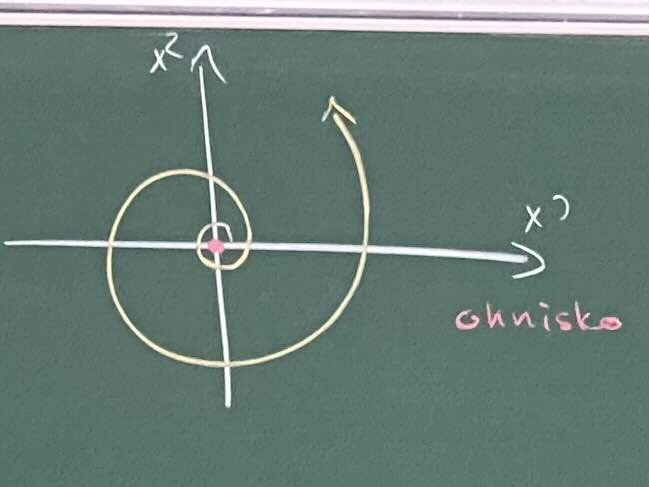
\includegraphics[width=0.5\linewidth]{images/ohnisko.jpg}
    \end{center}

    Pevný bod $x^\star = [0,0]$ je nestabilní

\end{enumerate}
\end{example}


\begin{definition}
    Trajektorie z předchozího příkladu pojmenujeme

    \begin{enumerate}
        \item Sedlo 
        \item Střed 
        \item Uzel 
        \item Nepravý uzel 
        \item Ohnisko
    \end{enumerate}

\end{definition}


\begin{example}
    Nekonečně rozměrný dynamický systém:
    \begin{equation}
        \partial_t u = D\partial^2_{xx} u, v (0,\infty) \times (a,b)
    \end{equation}

    Okrajové podmínky $u|_{x=a} = 0, u|_{x=b} = 0$ a počáteční podmínky $u|_{t=0} = u_{ini}(x)$ v $(a,b)$


    ÚKOL: zapsat (pomocí RMF) analytické řešení ve tvaru řady a určit, jaký DS generuje. \todo{HW}
\end{example}

\begin{definition}
    Nechť $x^\star$ je pevný bod dynamického systému na $X$. Pak množina $\mathcal{M}_- (x^\star) = \left\{x_0 \in X| S(t)x_0 \overset{t\rightarrow\infty}{\longrightarrow} x^\star\right\}$ se nazývá \textbf{stabilní varieta}.
    
    Množina
    \begin{multline*}
    \mathcal{M}_+ (x^\star) = \{x_0\in X| (\exists \text{úplná trajektorie} \left\{u(t)\right\}_{t\in\mathbb{R}})\\(\exists t_0 \in \mathbb{R}) (x_0 = u (t_0) \wedge u(t) \overset{t\rightarrow - \infty}{\longrightarrow} x^\star)\}
    \end{multline*}
    se nazývá \textbf{nestabilní varieta}.

    Nechť $A\subset X$ je invariantní a 
    \begin{equation*}
    \left(\exists B_0 \subset X, B_0 \in \mathcal{J}_x, B_0 \supset A\right) \left(\forall x_0 \in B_0\right) \left(\varrho(S(t)x_0, A) \overset{t\rightarrow\infty}{\longrightarrow} 0\right)
    \end{equation*}
     pak $A$ se nazývá \textbf{atraktor}.

\end{definition}


\begin{remark}
    Trajektorie $\{u(t)\}_{t\in\mathbb{R}}$ je úplná, když je 
    parametrizovaná $\forall t \in \mathbb{R} (t \in \mathbb{R} \cap\mathbb{Z})$, tj $t$~lze~$\binom{\rightarrow + \infty}{\rightarrow - \infty}$. 
    To \textbf{neznamená}, že diskrétní systém musí být invertovatelný.

    Atraktory jsou asymptoticky stabilní pevné body a mnohem více (viz. dále).
\end{remark}


\end{document}